\section{Dynamic Optimization}\label{DO}

When engineers speak about optimization, they usually refer to static optimization, in which the optimization variables p are finite, also called parameters (e.g., finding the most efficient operating point of an engine). Then optimal refers to some well-defined optimization criterion, usually the minimization of a cost function J(p) (e.g., fuel consumption per hour). 
Trajectory optimization is different in that the optimization variables are functions x(t) of an independent variable t, usually time. It is also called dynamic or infinite-dimensional optimization. Evaluating x(t) therefore requires a cost functional (a “function of a function”), which quantifies the “quality” of the trajectory x(t) by a scalar value. 
Due to the vehicular focus, a special case will be considered, one that requires the trajectory x(t) to be consistent with some dynamical system model which has an input u. Without such model, the optimization cannot incorporate the inherent properties and physical limitations of the vehicle. This special case of dynamic optimization is called an optimal control problem (e.g., Lewis and Syrmos 1995).

\subsection{Optimal Control Problem}
A fairly general formulation of the optimal control problem (OCP) reads:

%% TODO Formulas

Minimize the cost functional
% J(u(t))= ∫_0^(t_f)▒〖l(x(t)  ,u(t),t)  "d" t〗+V(x(t_f ),t_f )	(57.1))

subject to the system dynamics
% x ̇(t)=f(x(t),u(t),t),    x(0)=x_0	(57.2))
as well as the equality and inequality constraints

% g(x(t_f ),t_f )=0 and	(57.3))
%h(x(t),u(t),t)≤0 for all times on the interval [¬0,t_f ].	(57.4))

In other words, for our (possibly nonlinear and time variant) system with state %x∈R^n 
and input %u∈R^m  
we seek on the interval %t ∈[¬0,t_f ] 
the input trajectory u(t) that minimizes the cost functional J while steering (in the truest sense of the word) the system from its initial state $x_0$ to an end state $x(t_f )$, so that the equality and inequality constraints are fulfilled at all times. The optimal input trajectory is usually denoted by 
%u^* (t) 
and the resulting state trajectory by %x^* (t), 
see Fig. \ref{fig:dynamische_Optimierung_endvorgabe}. Notice that J comprises integral costs l and end point costs V and is not only a functional of the input u(t) but also of the states x(t). Furthermore, if the final time $t_f$ is not given, it then becomes part of the optimization, so that the length of the trajectory will also be optimized.

\begin{figure}[h]
\psfrag{1}[cr][cr][1.0]{$x_1$}
\psfrag{2}[br][br][1.0]{$x_2$}
\psfrag{x}[tc][tc][1.0]{$\bs{x}^\ast(t)$}
\psfrag{0}[cr][cr][1.0]{$\bs{x}_0$}
\psfrag{e}[tl][tl][1.0]{$t_f$}
\psfrag{o}[tl][tl][1.0]{$0$}
\psfrag{t}[bc][bc][1.0]{$t$}
\psfrag{g}[bc][bc][1.0]{$\bs{g}=\bs 0$}
\psfrag{h}[tc][tc][1.0]{$h>0$}
	\centering
  	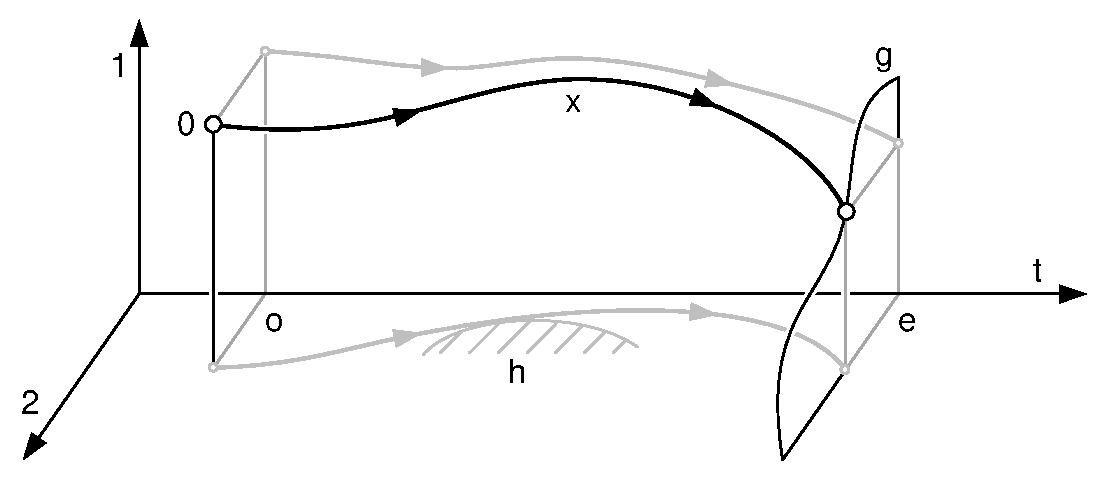
\includegraphics[width=1.\textwidth,clip, trim = 0cm 0cm 0cm 0cm]{pics/2_Darstellung_dynamische_Optimierung_endvorgabe.eps}
  	%\caption{Figure 1} %[Veranschaulichung der Lösung des Optimalsteuerungsproblems]{Veranschaulichung der Lösung $\bs{x}^\ast (t)\in \mathbb{R}^2$ eines Optimalsteuerungsproblems mit Endbedingung $\bs{g}=\bs 0$ und Ungleichungsbeschränkung $h\leq 0$ für $x_2$ sowie fester Endzeit $t_f$}
    \label{fig:dynamische_Optimierung_endvorgabe}
\end{figure}

\subsection{Problem Formulation for DAS and Automated Driving}
Coming back to the automotive application, equation (2) of the previous section describes the dynamics of the vehicle. This state space model also includes the planar motion, either relative to some reference such as the lane center, see Sect. 57.3.1.2, or relative to a stationary origin, see Sect. 57.3.3.4. Undesired vehicle motion such as deviations from the lane center, detours, dangerous vehicle states (e.g., large slip angles), or uncomfortable jerks, e.g., caused by hectic steering actions will be penalized in the cost functional (1). The free space prediction between the generally moving obstacles can be described by the inequality constraints (4). And the end constraints (3) can be utilized to require that the optimized vehicle trajectory will be aligned to the road at the end of the optimization interval. As will be explained in Sect. 57.5, this final state plays an important role for the stability of the “replanning” algorithm, therefore special costs
%V(x(t_f ),t_f )
can be introduced in (1). 

\subsection{Solving the Optimal Control Problem}

\subsubsection{Approach I: Calculus of Variations}
The classical approach to the OCP is calculus of variations, which delivers valuable insight in the solution. 

Theoretical Background: Hamilton Equations

Static optimization problems can be tackled by differential calculus. It is well known that the first derivative of a function J(p) is equal to zero at a minimum (or any other stationary point). For multivariate problems we can write 
%∇J(p)=0, 
which leads to a set of (algebraic) equations that the optimum 
%p^* 
must satisfy. The extension to problems with equality constraints requires the method of so-called Lagrange-multipliers, yielding first order necessary conditions for optimality.
Analogously for dynamic optimization, variational calculus requires that the first variation of the functional %J(u(t)) 
vanishes for the optimal control function %u^* (t), 
which is often written as 
%δJ(u(t))=0. 

In order to incorporate the system dynamics in the OCP, which constitute (differential) equality constraints, we can also apply the Lagrange-multiplier method. This yields a set of differential equations, the so-called Hamilton equations:

%x ̇=f(x,u,t)	(57.1))
%λ ̇=-∂l/∂x-[∂f/∂x]^"T"  λ	(57.2))
%0=-∂l/∂u-[∂f/∂u]^"T"  λ

They are first order necessary conditions for our OCP, when there are no inequality constraints (4) involved. The function 
%λ(t) 
constitutes the Lagrange-multipliers, here called co-states. Besides the initial condition
%x(0)=x_0	(57.1))
the optimal trajectory must fulfill the (algebraic) transversality conditions, depending on whether the end state 
%x(t_f) 
is constraint by (3) and/or the final time 
%t_f 
is given (see e.g. (Lewis and Syrmos 1995)). The simplest condition requires a fixed end state 
%x_f
at a given end time 
%t_f
so that
%x(t_f  )=x_f.	(57.2))
Either way, this results in a boundary value problem, which in general needs to be solved numerically. This so-called indirect approach is very accurate but not as flexible as the direct approach that we will introduce in Sect. 57.3.2. However, for simple OCPs the resultant boundary value problem can be solved analytically, leading to fast computable optimal trajectory primitives with broad applications (see Sect. 57.4).

57.3.1.2	Example Application: Automated Lane Change

We will now apply the described method to the generation of optimal lane change primitives. The lateral motion across the road can be modelled as a triple integrator system with states 
%x=[x_1,x_2,x_3 ]^"T" , 
namely the position, the lateral velocity, and the lateral acceleration, respectively, all within the reference frame of some curve, see Fig. 57.2.
Then, the system dynamics are described by 
%x ̇=f(x,u)=[x_2,x_3,u]^"T" ,	(57.1))
where u represents the lateral jerk, which is the third derivative of the lateral position. We will now seek for the optimal system input %u^* (t)  
that transfers the integrator system from its initial state
%x(0)=x_0	(57.2))
 to a given end state 
%x(t_f  )=x_f	(57.3))
at a given end time 
%t_f. 
Amongst all trajectories we seek for the one that minimizes the integral of the jerk-square, that is
%l=1/2 〖u(t)〗^2,

so that the movement feels most pleasant to the passengers. Notice that the final cost here has no influence on the solution due to the fixed end state, so that we can set V=0 in (1).
With 
%λ=[λ_1,λ_2,λ_3 ]^"T" , 
evaluating the so-called control equation (7) we obtain
%0=u+ λ_3   □(⇒)  u= -λ_3  .	(57.1))
The co-state equation (6) yields
%λ ̇=[λ ̇_1,λ ̇_2,λ ̇_3 ]^"T" = [0,〖-λ〗_1,〖-λ〗_2 ]^"T" 	(57.2))
and therefore, we get
%〖  ⇒ λ〗_1:=〖-c〗_1,〖   λ〗_2=c_1 t+c_2,"and " λ_3=-1/2 c_1 t^2-c_2 t-c_3 " ." 	(57.3))
With 
%λ_3 
from (16) it can be seen from (14) that the optimal control input function is a third order polynomial with yet unknown integration constants 
%c_1,c_2, and c_3. 
Substituting 
%u(t)
in the state equation (10) we find the optimal trajectory to be
%  x ̇_3= -λ_3    ⇒x_3 (t)=  1/6 c_1 t^3+1/2 c_2 t^2+c_3 t+c_4	(57.4))
%  x ̇_2= x_3    ⇒x_2 (t)=  1/24 c_1 t^4+1/6 c_2 t^3+〖1/2 c〗_3 t^2+c_4 t+c_5	(57.5))
%  x ̇_1= x_2    ⇒x_1 (t)=  1/120 c_1 t^5+1/24 c_2 t^4+〖1/6 c〗_3 t^3+〖1/2 c〗_4 t^2+c_5 t+c_6	(57.6))
with additional integration constants %c_4,c_5, and c_6. 
To comply with the initial state (11) and end constraint (12) the integration constants need to be chosen accordingly. As (16)-(19) are linear with respect to the constants this can be done by simple linear algebra, leading to the trajectory (a) in Fig. 57.2. 
Similarly, we can find the solution to the OCP with a free end state (and a free end time). In this case we require the end state to be as close to (and as soon at) the reference as possible by setting
%V(x)= k_1 x_1 (t_f )^2+k_2 x_2 (t_f )^2+k_3 x_3 (t_f )^2,〖 k〗_i>0 
%(V(x)= 〖k_t t〗_f+k_1 x_1 (t_f )^2+k_2 x_2 (t_f )^2+k_3 x_3 (t_f )^2,〖 k_i,k〗_t>0)	
The new transversality conditions will only lead to a different end state and end time, see (b) and (c) in Fig. 57.2. However, the optimal function class, that is the 5th-order polynomial, will stay the same.

Fig. 57.2 Optimal lane changes for (a) a given end time and end state; (b) a given end time and a free end state; (c) a free end time and a free end state


57.3.1.3	Further Readings
The previous calculations can be analogously carried out for the longitudinal movement, which leads to a very comfortable braking characteristic (Gutjahr and Werling 2014). The longitudinal and lateral movements can also be combined by a regular local and temporal sampling of target states across and along the street. This leads to a reactive algorithm which prevents collisions with static and moving obstacles (Werling et al. 2012).
The variational approach was generalized to problems with input constraints, known as Pontryagin's minimum principle. As for the vehicular application, it yields the shortest path connecting two poses of 
a vehicle with a limited turn radius (Dubins 1957; Reeds and Shepp 1990; Boissonnat et al. 1994). Even more involved is finding variational solutions to problems with state constraints such as the optimal braking application in Fig. 57.3. (e.g., Bryson and Ho 1975).
Numerical solutions to the first order necessary conditions can be found by so-called indirect methods (see e.g. Graichen 2012) which provide very accurate results in general. Contrary to direct methods, as described in the sequel, they need to determine initial conditions for the co-states, which has made the applications unsuitable for an automotive online application yet.

Fig. 57.3 Minimal jerk-square minimal time stopping trajectories with acceleration constraint 
%a≥10 "m"/"s" ^2

\subsubsection{Approach II: Direct Optimization Techniques}
Direct optimization is probably the most widely explored approach in model-predictive control. It approximates the dynamic optimization problem of the OCP to a static one, as the latter can be efficiently solved by well-established numerical solvers. The essence of this approach is a finite-dimensional parameterization of the input, state, or output trajectory.





